\subsection{Deployment paths}
\label{subsec-deployment}
\cappos{Needs to be less implementation specific and more general...}

% Fraidy: I do not like this idea of an "uncooperative"
% application. I also want to focus more on "who" rather 
% than "where"

% There are two orthogonal concerns when deploying Affix with an 
% application: \textit{Cooperation} -- the application might or 
% might not actively expect and liaise with the Affix framework --, 
% and \textit{location} -- Affix components can be deployed at 
% different elements along the network path.

% A cooperative, i.e. Affix-aware, application includes Affix 
% functionality natively by using the  Affix libraries, so that 
% users will benefit without having to explicitly load Affix
% stacks on their own. An uncooperative application can be 
% forced to use Affixes either by relaying its traffic through 
% an Affix-aware \textit{proxy} application (on the same host, or 
% on a separate middlebox), 
% or by \textit{interposition} on its network library calls, 
% e.g. by setting the \texttt{LD\_PRELOAD} variable in Linux so that 
% Affix functions will be used before those of the same name in 
% the standard libraries. 
% Either way, program behavior is modified non-invasively, 
% and it can be configured system-wide 
% or used selectively on a per-application basis.


The Affix framework and core services may be installed as a 
Python package. Once installed, 
there are several methods available for using 
Affix, including:
\begin{itemize}
    \item \emph{Proxy}-based use. The Affix package includes a Python proxy,
which can load an abitrary Affix configuration. 
Traffic must be tunneled through the 
proxy for Affix functionality to be applied.
    \item \emph{Interposition}. The Affix library may interpose on network library calls 
(e.g., by setting the \texttt{LD\_PRELOAD} variable in Linux) so that 
its functions will be used before those of the same name in the standard libraries. 
    \item \emph{Native} integration within an application. A developer can 
choose to include Affix functionality natively in an application using the Python 
library.
\end{itemize}
The first two cases are suitable where the source code of an application 
is not available, where native integration is not practical, and/or when 
Affix is deployed by a non-programming end user.
In both proxy- and interposition-based use, 
program behavior is modified non-invasively, and it can be configured system-wide 
or used selectively on a per-application or per-socket basis.
\cappos{I thought ``How?'' when reading here.   Maybe describe a decider 
component in a sentence.}


% Albert: How about \multirow's and sub-figures?
\begin{figure*}[t]
  \centering
  \begin{tabular}{c c c c}  
  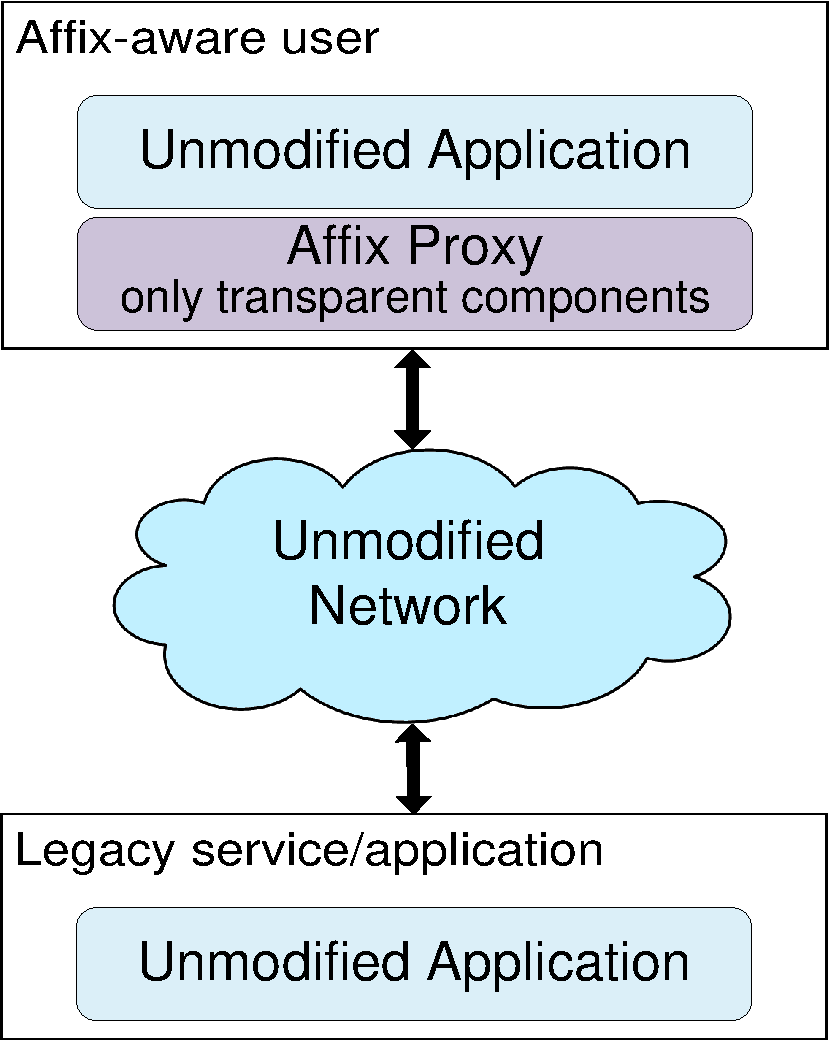
\includegraphics[height=4.75cm]{figs/dep3.pdf} \hspace{.05cm} &
  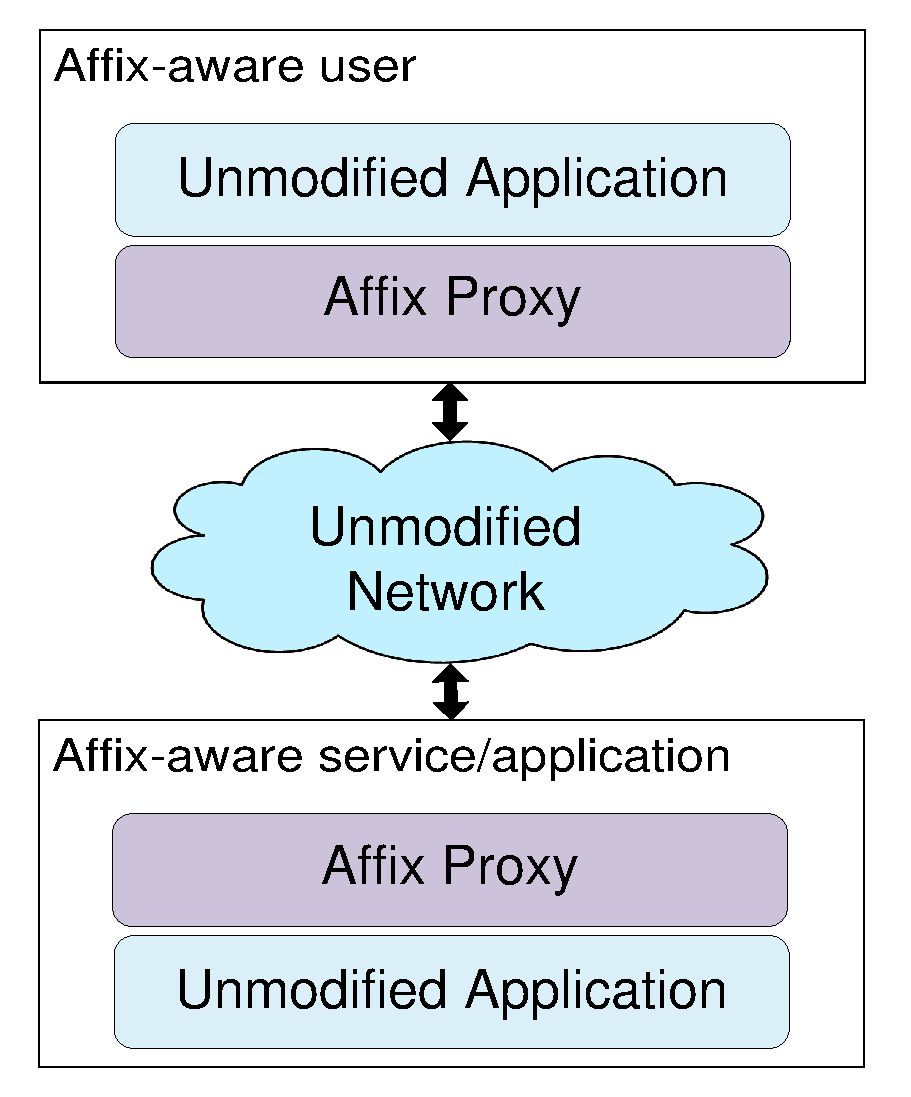
\includegraphics[height=4.75cm]{figs/dep2.pdf} \hspace{.05cm} &
  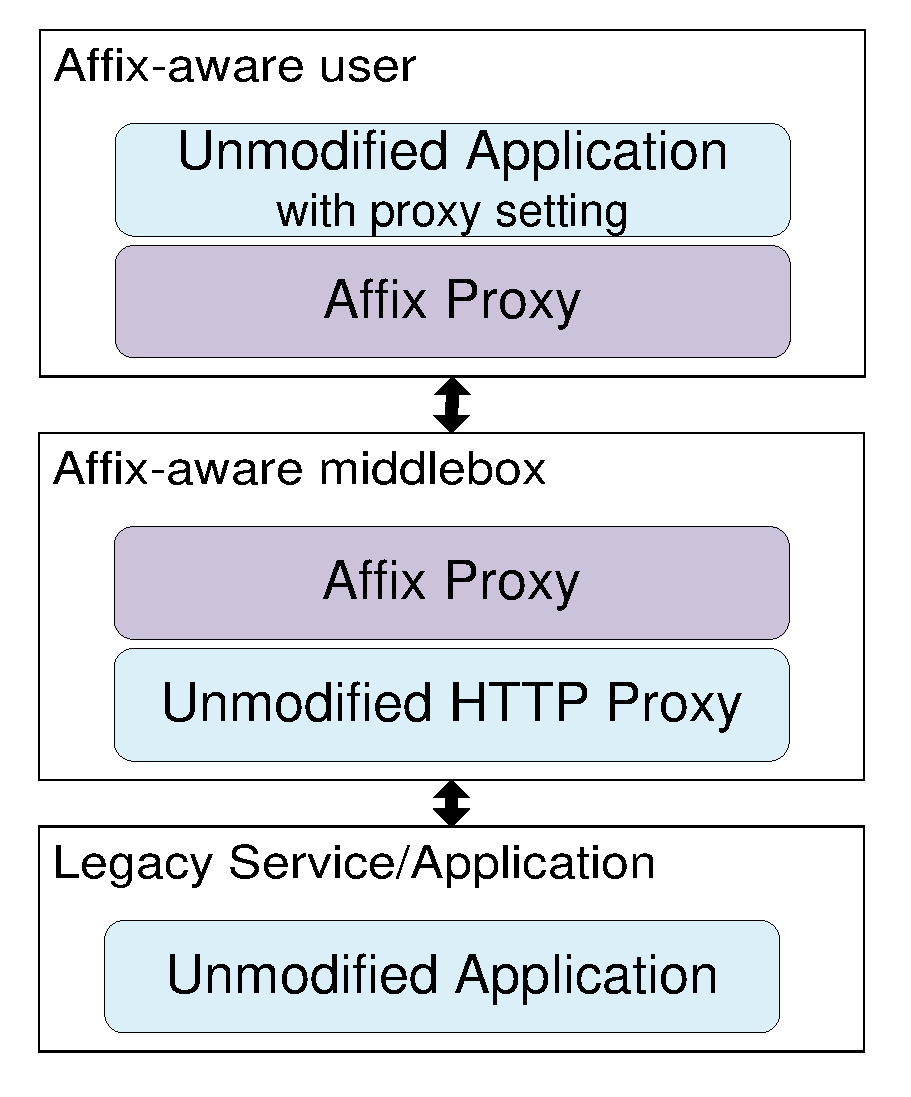
\includegraphics[height=4.75cm]{figs/dep1.pdf} \hspace{.05cm} &
  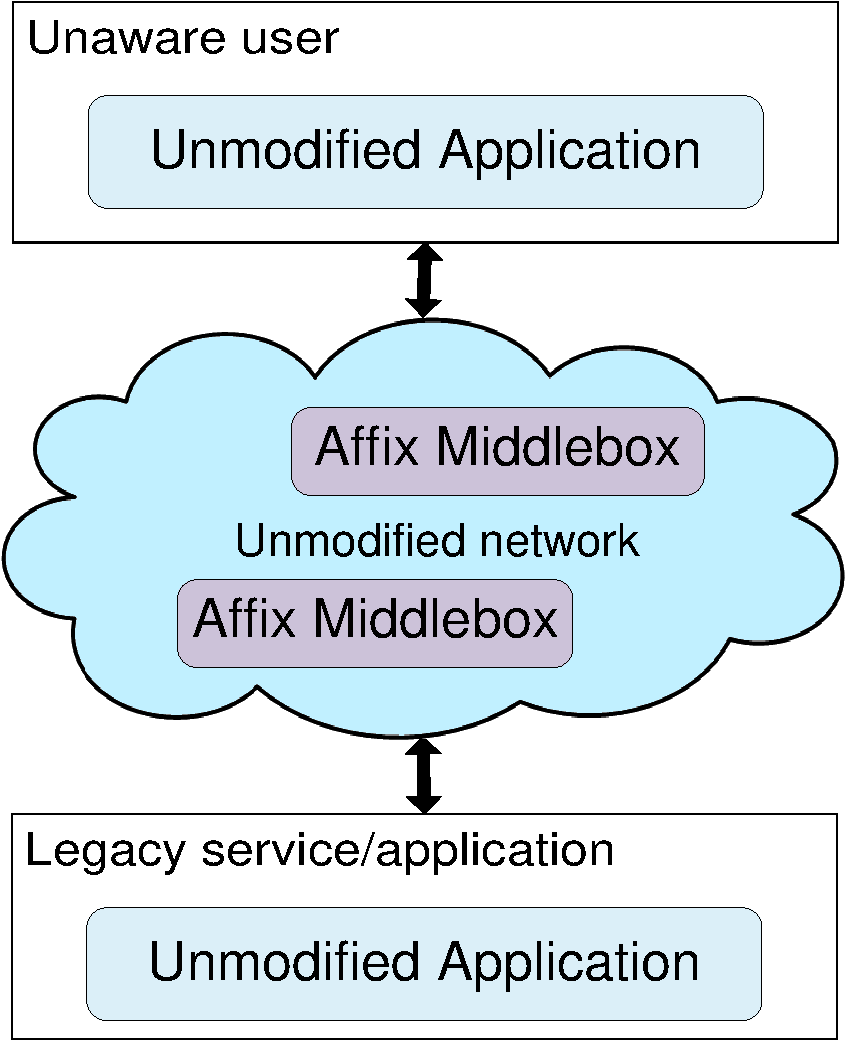
\includegraphics[height=4.75cm]{figs/dep4.pdf} \\
  (a) Only user is  \hspace{.05cm} & (b) User and service \hspace{.05cm} &  (c) User and middlebox \hspace{.05cm} &  (d) Only the core network \\
  Affix-aware  \hspace{.05cm} & are Affix-aware \hspace{.05cm} &  are Affix-aware \hspace{.05cm} &  is Affix-aware
\end{tabular}
  \caption{Affix supports various deployment paths for unmodified applications, depending on which parties are involved. Note that it is possible to use Affix if only the end user is 
  Affix-aware, as shown in Figure~\ref{affix-deployment}(a), 
  as well as when neither end user nor web service provider are Affix-aware, 
  as in Figure~\ref{affix-deployment}(d).   Applications co-located with
an Affix proxy may alternatively be changed to natively support Affix.}
  \label{affix-deployment}
\end{figure*}


Figure~\ref{affix-deployment} shows four possible deployment 
options available for use with unmodified applications
(i.e., the application developer is not a cooperating party). 
These deployment options are especially 
important in the context of democratic deployment, 
and several are unique to the Affix framework:

\begin{itemize}
    \item A user can run an Affix proxy to use transparent 
Affix components (such as rate limiting), and tunnel traffic from applications 
through the proxy, as in Figure~\ref{affix-deployment}(a),
    \item Users on two sides of a connection can run the 
proxy with double-sided Affix components (such as compression or encryption),
and tunnel traffic from applications through the proxy, as in Figure~\ref{affix-deployment}(b),
    \item A user can run the included Affix proxy to use double-sided and single-sided
Affix components, and direct traffic from applications to a proxy elsewhere on 
the Internet that offers Affix functionality, as in Figure~\ref{affix-deployment}(c)
    \item Traffic can be routed through an Affix stack without deploying 
    Affix on any end devices, by applying the interposition 
method on middlebox devices as in Figure~\ref{affix-deployment}(d).
%    \item An operating system can use the interposition method to 
%support Affix functionality with every application,
%    \item An application developer can use Affix components directly 
%within an application,
%    \item An advanced user or application developer can use Affix components 
%directly in a wrapper around an application.
\end{itemize}
